\chapter{Estado del Arte}

Las competencias de drones autónomos han adquirido un grado alto de relevancia en la última década, dentro del marco teórico del presente trabajo se describe con profundidad el contexto histórico, así como la motivación y los requerimientos establecidos para tres de las competencias, más significativas de drones autónomos; el  IROS Autonomous Drone Race, el AlphaPilot AI Drone Innovation Challege y el Game of Drones. 

En este capítulo se presentan algunas de las soluciones propuestas en estas competencias, al igual que trabajos con enfoques más prácticos o que no se encuentran directamente relacionados con las carreras de drones autónomos.

Dentro de las competencias anteriormente mencionadas, existen dos problemas esenciales a los que se enfrentan los equipos que participan en estos retos, la detección de objetos y la gestión de trayectoria de vuelo a partir de la detección realizada. 
Los circuitos que tiene que completar los drones están definidos por compuertas de distintas formas y tamaños, y en algunos casos se adicionan obstáculos dinámicos. Los vehículos desarrollados por los participantes tienen que ser capaces de detectar estos objetos haciendo uso exclusivo de sensores abordo del dron (cámaras, sensores ultrasónicos, tecnología láser, etc.).

Con base en lo anterior, \citet{cabrera2019gate} desarrollaron un algoritmo para la detección de compuertas en tiempo real utilizando aprendizaje profundo. Su implementación se basó en una arquitectura de red neuronal convolucional (RNC) con una arquitectura similar a la Single Shot Detector de 7 capas, \citet{SSD7}. La arquitectura base tiene un diseño optimizado para la detección de objetos, permitiendo un tiempo de entrenamiento reducido y una velocidad de detección alta; esta se modificó de tal forma que se eliminaron las últimas dos capas de convoluciones, haciendo posible una detección mucho más rápida que la propuesta base y disminuyendo la complejidad de la red. El entrenamiento de la red se realizó con un total de 3418 imágenes obtenidas a partir de un entorno simulado y entornos reales. 
Además, para observar el desempeño de su implementación compararon su arquitectura con otras propuestas, SSD7, SSD300 y SmallerVGG, en simulaciones y ambientes de exteriores e interiores. Los resultados muestran que su propuesta logra un tiempo de detección promedio más bajo y porcentaje de confianza más alto que las otras arquitecturas. 

La figura \ref{fig:SSD} muestra algunos de los resultados obtenidos por \citet{cabrera2019gate}, en el conjunto de imágenes se logra apreciar la influencia que tienen los datos de entrenamiento utilizados sobre el desempeño obtenido; el primer tercio de imágenes, las del extremo izquierdo, se obtienen a partir de un entrenamiento basado exclusivamente en imágenes de simulación; los resultados de la parte central fueron obtenidos entrenando la red con imágenes de compuertas reales, y por último, el último conjunto de resultados se obtuvo combinando imágenes de simulación e imágenes reales para el entrenamiento. Como es posible apreciar, la RNC tuvo un mejor desempeño al entrenarla con imágenes capturadas en simulación e imágenes de un ambiente real.

\begin{figure}[ht]
    \centering
    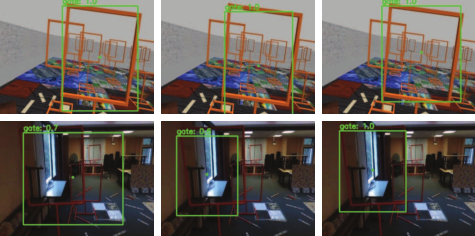
\includegraphics[width=0.8\textwidth]{SSD.pdf}
    \caption{Validación del algoritmo de detección de compuertas basado en SSD7 \citet{cabrera2019gate}}
    \label{fig:SSD}
\end{figure}

Por otro lado, \citet{mellinger2011minimum} presentaron un diseño de control y generación de trayectoria de vuelo en ambientes de interiores para un quadrotor. Su implementación es capaz de generar una trayectoria óptima y ángulos para la guiñada del vehículo, en tiempo real, a partir de matrices de rotación para el marco de referencia del vehículo y una secuencia de posiciones en tres dimensiones. La propuesta fue diseñada con el objetivo de que el quadrotor sea capaz de navegar de forma segura a través de corredores angostos, manteniéndose en los límites de velocidad y aceleración. Además, implementaron un control no lineal que asegura el seguimiento de las trayectorias generadas; las propuestas se pusieron a prueba con un prototipo físico  que se hizo volar a través de un circuito construido por aros, los cuales indicaban la trayectoria que el quadrotor debía de seguir. La figura \ref{fig:MinimumSnapTrajectory} muestra el recorrido realizado por el dron durante una de las pruebas.

\begin{figure}[ht]
    \centering
    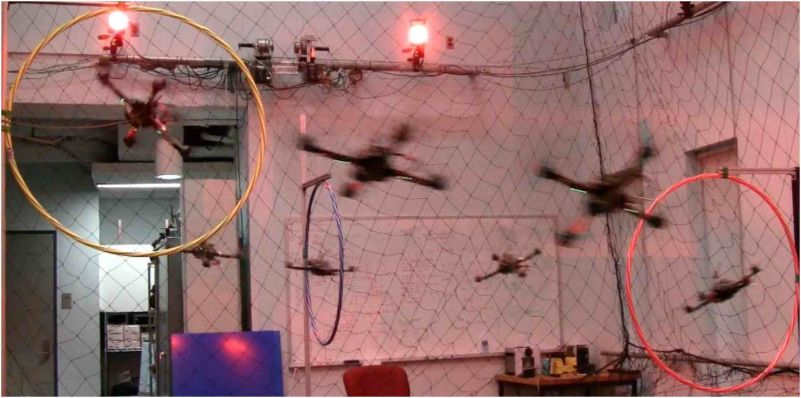
\includegraphics[width=0.8\textwidth]{MinimumSnapTrajectory.pdf}
    \caption{Imagen compuesta del vuelo del dron \citet{mellinger2011minimum}}
    \label{fig:MinimumSnapTrajectory}
\end{figure}

Adicionalmente, Mueller et al.(2013)\citet{mueller2013computationally} diseñaron un algoritmo de bajo consumo computacional para la generación de trayectorias de intersección para la ruta de vuelo de un quadrotor. La implementación tuvo como propósito que el quadrotor fuera capaz de interceptar una pelota en vuelo, con una raqueta montada en su chasis, la figura \ref{fig:mueIROS13} muestra el dron utilizado. El algoritmo de generación de trayectoria se usó en un sistema de control predictivo, en donde miles de trayectorias eran generadas y evaluadas al mismo tiempo, y después, la trayectoria más óptima era seleccionada por el algoritmo.  Se destaca el bajo coste computacional pues se utilizó el hardware de una laptop estándar para evaluar cerca de un millón de trayectorias por segundo.

\begin{figure}[ht]
    \centering
    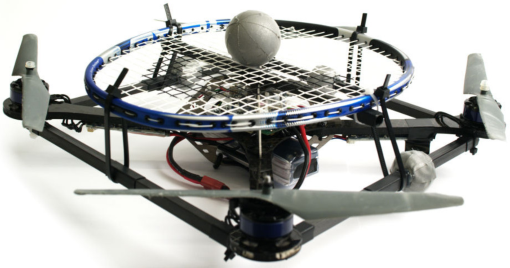
\includegraphics[width=0.6\textwidth]{mueIROS13.pdf}
    \caption{Dron con raqueta incorporada \citet{mueller2013computationally}}
    \label{fig:mueIROS13}
\end{figure}

Las propuestas anteriores representan ejemplos de soluciones individuales para cada uno de los problemas mencionados. Sin embargo, existen implementaciones que solucionan ambos problemas en un solo trabajo, y corresponden a aquellos sistemas que fueron desarrollados para participar en las competencias.

El trabajo realizado por \citet{moon2019challenges} compila una serie de propuestas destacadas, y describe con detalle los algoritmos de visión artificial, odometría, control de vuelo, etc., desarrollados para el IROS 2017 por los equipos más sobresalientes de la competencia. 

Se presentan 5 propuestas distintas. Iniciando por el equipo ganador de la competencia, los participantes del Instituto Nacional de Astrofísica, Óptica y Electrónica (INAOE); implementaron un control PID para la altura, curso y ángulo de deslizamiento del dron; además, obtuvieron la localización espacial del dron y su orientación a partir de un algoritmo de  deep learning basado en ORB-SLAM. Su algoritmo de odometría asume que el suelo de la pista es plano, por lo que al conocer la altura y ángulo de la cámara de vuelo, les fue posible generar una trayectoria de vuelo adecuada para el cruce de las compuertas. La figura \ref{fig:ISR19_Moon} presenta la participación del equipo INAOE, en donde se logra observar la implementación de su algoritmo de detección, su sistema de odometría y su propuesta para la generación de trayectorias de vuelo.

\begin{figure}[ht]
    \centering
    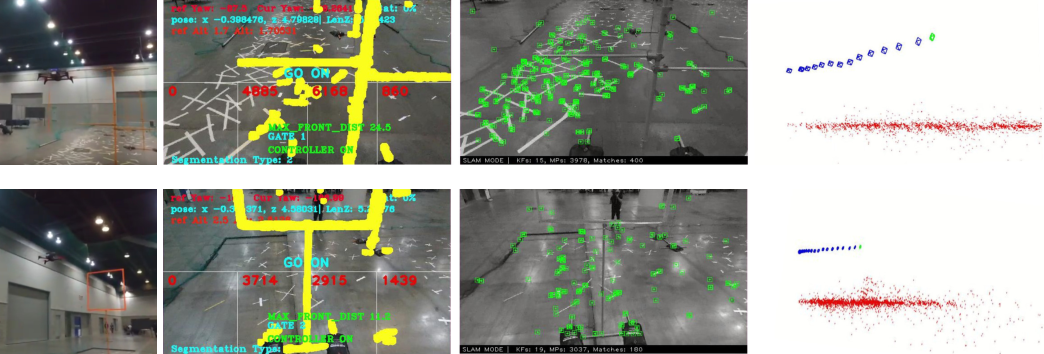
\includegraphics[width=0.8\textwidth]{ISR19_Moon.pdf}
    \caption{Imagen compuesta del vuelo del dron del equipo INAOE\citet{moon2019challenges}}
    \label{fig:ISR19_Moon}
\end{figure}


Por otro lado, el equipo de la Universidad de Zúrich (UZH) propuso una solución basada en la elaboración de un modelo 3D del circuito de vuelo, el cual utilizó para definir una serie de waypoint para la navegación del dron; a cada waypoint se le asoció un vector de velocidad. Lo anterior, en conjunto con un sistema de odometría visual, permitieron que el dron del equipo de UZH navegara de forma autónoma a través del circuito. 
El principal reto para esta implementación fue la alineación de la pista con el marco de referencia del dron, para solucionarlo, utilizaron  un sensor de profundidad junto con un mapa de referencia, de tal forma que minimizan la distancia entre la nube de puntos de la pista y el conjunto de puntos proveídos por el sensor.

El tercer lugar del IROS 2017, le perteneció a la Universidad Técnica de Delft (TU Delft). Este equipo buscó enfocar su propuesta en drones de tamaño compacto ($<$ 50 cm), teniendo como objetivo un vuelo rápido, ágil y de bajo costo computacional. Lo anterior contempla ciertas limitaciones inherentes en cuanto a la cantidad de sensores integrados en el vehículo y la gama de la computadora de vuelo que se puede utilizar.
Dicho esto, el equipo TU Delft optó por utilizar una máquina de estados para la gestión de la trayectoria de vuelo, en donde cada estado está asociado a un comportamiento específico definido para cada parte del circuito; esto representa una ventaja, pues la máquina de estados es muy eficiente, computacionalmente hablando. 
Por otro lado, la máquina de estados necesita la posición y orientación del dron con respecto a la compuerta que está a punto de cruzar; la detección de compuerta se realizó utilizando un algoritmo basado en la detección del color de estas; es decir, no utilizaron RNC por el alto consumo de recursos, y en su lugar hicieron uso de funciones básicas de visión artificial para realizar una segmentación del color de la compuerta, y de esta forma realizar su detección. A partir de lo anterior, se detectó las esquinas de las compuertas, y utilizando la geometría conocida de las mismas, fue posible determinar la posición y orientación con respecto a la compuerta. Adicionalmente, el equipo implementó una detección basada en un histograma de colores, el cual detecta los vértices que considera más verticales para detectar la compuerta más cercana, y a diferencia del algoritmo anterior, esta propuesta esta pensada para realizar la identificación cuando no toda la compuerta es visible, por lo que ambos algoritmos se complementaron para realizar la detección de las compuertas. 

En la figura \ref{fig:ISR19_Moon1} se muestran algunas capturas realizadas durante la participación del equipo; en ellas se aprecia la precisión obtenida para la detección de compuertas. En la primera columna de imágenes se observa el algoritmo de detección por color, mientras que en la segunda columna se aprecia las barras verticales producto del algoritmo con el histograma de colores. Por último, la imagen de la tercera columna muestra el dron del equipo Tu Delft cruzando a través de una compuerta de forma autónoma.

\begin{figure}[ht]
    \centering
    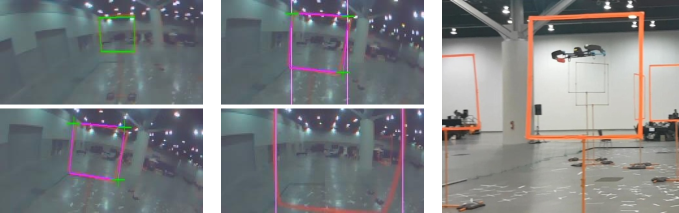
\includegraphics[width=0.8\textwidth]{ISR19_Moon1.pdf}
    \caption{Resultados de la implementación del equipo TU Delft \citet{moon2019challenges}}
    \label{fig:ISR19_Moon1}
\end{figure}

Después, el equipo del Instituto Avanzado de Ciencia y Tecnología de Corea (KAIST) propuso una combinación de una arquitectura de deep learning para la detección de compuertas y un algoritmo de guía por línea de vista (Line Of Sight Guidance) para la generación de la trayectoria de vuelo.
 El equipo KAIST implementó una RNC de 7 capas convolucionales, basada en la arquitectura de ADRNet, para el procesamiento de imágenes y la detección de compuertas en tiempo real. Esta arquitectura logró la inferencia a una velocidad de 28.95 fps en una computadora de placa única NVIDIA TX2. 
Por otro lado, KAIST logró la generación de maniobras precisas para el pase a través de compuerta con un algoritmo de tipo Line of Sight Guidance. Este algoritmo es muy utilizado en aeronaves de ala fija, y fue modificado ligeramente para que se adaptara a la dinámica de un quadrotor.
La propuesta desarrollada por KAIST representa un buen acercamiento para navegar en situaciones de alta incertidumbre, pues no depende del mapa del circuito; sin embargo, lo anterior es ineficiente, en circuitos donde se conocen los detalles y composición del recorrido de vuelo, a priori.

Por último, en cuanto al IROS 2017, el equipo de la Universidad Nacional de Ulsan (UNIST) implementó una red neuronal profunda para la detección de las compuertas del circuito, y a partir del procesamiento de las imágenes, lograron generar controles de vuelo para el desplazamiento horizontal, vertical y las acciones rotacionales. Los comandos de vuelo son generados en forma de un mensaje de tipo MAVLink para que la computadora de vuelo los pueda interpretar, controlando el dron de forma directa.
La arquitectura de la red neuronal está basada en la red Google Inception de \citet{xia2017inception}, la cual representa el estado del arte de las arquitecturas para detección y clasificación. 
Bajo esta implementación, el dron es capaz de volar a través de las compuertas con dos pasos; el dron se encuentra en una posición inicial y su cámara tiene que tener en su campo de visión a la compuerta a atravesar; se establece una línea recta con respecto al centro de la compuerta y el dron vuela tomando esa trayectoria como referencia. Una vez alineado con la recta, el dron vuela a través del centro de la compuerta. La figura \ref{fig:ISR19_Moon2} muestra un diagrama general de los pasos descritos anteriormente para la implementación del equipo UNIST.

\begin{figure}[ht]
    \centering
    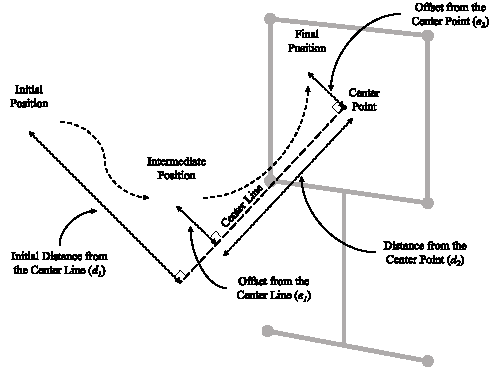
\includegraphics[width=0.6\textwidth]{ISR19_Moon2.pdf}
    \caption{Propuesta desarrollada por el equipo UNIST, \citet{moon2017iros}}
    \label{fig:ISR19_Moon2}
\end{figure}


A partir de lo anterior, es evidente el impacto y la importancia que han adquirido las redes neuronales profundas dentro de las competencias de drones autónomos. Otro ejemplo de este tipo de implementación fue presentado por \citet{kaufmann2018deep};  desarrollaron un sistema de visión artificial y seguimiento de trayectoria, pensado para ambiente dinámicos, en donde se requiere de un vuelo ágil y una estimación de estados adecuada, que permita una rápida y correcta definición de la trayectoria de vuelo para el dron. 
Para lograrlo, implementaron una RNC basada en la RedNet de \citet{loquercio2018dronet}, acoplada a un algoritmo de planificación de trayectoria; la red neuronal recibe imágenes directamente de la cámara de vuelo del dron y realiza un mapeo de tal forma que genera un waypoint y una referencia de velocidad deseada, lo cual es utilizado posteriormente por un algoritmo planificador para generar el segmento de trayectoria más corto y los comandos para los motores, de tal forma que el dron pueda alcanzar su destino. Esta implementación no requirió del conocimiento previo del circuito de vuelo, pues todos los cálculos son realizados en tiempo real durante el vuelo. Esta propuesta se implementó en simulación y en un ambiente físico en donde algunas de las compuertas del circuito cambiaban de posición durante el vuelo, además, su desempeño se comparó con el obtenido con un vuelo realizado por pilotos con distinta experiencia de vuelo. Los resultados muestran que este sistema tuvo un desempeño más bajo en comparación con la habilidad y destreza de los pilotos humanos; sin embargo, este sistema ejemplifica una buena implementación de un algoritmo de percepción robusto en conjunto con una arquitectura moderna de machine learning y algoritmos de velocidad y estabilidad de vuelo. 

Por otro lado, \citet{rojas2020deeppilot} presentaron una propuesta bastante llamativa. Presentaron una arquitectura de RNC para procesar imágenes obtenidas a partir de una cámara montada en el dron y generar comandos de vuelo que permiten que el dron centre su trayectoria y pase a través de compuertas de un circuito de vuelo similar al de la competencia del IROS. Utilizaron una ambiente de simulación elaborada en Gazebo para la obtención de datos para su entrenamiento y validación de su sistema. Como parte de su contribución, propusieron una nueva arquitectura de RNC, que toma como entrada un mosaico de imágenes compuesto por un arreglo de tomas capturadas por la cámara del dron durante su vuelo, lo anterior permite tener cierta temporalidad del comportamiento del dron y deducir la acción de vuelo más adecuada para cruzar a través de una compuerta.
Además, utilizaron ROS para la gestión de los procesos en la computadora de vuelo y se hace la comparación con la arquitectura de otras RNC. La figura \ref{fig:Rojas_Perez} muestra un diagrama general de la implementación de \citet{rojas2020deeppilot} en 4 pasos; primero se adquiere la imagen captada por la cámara del dron; después, se utiliza la imagen captada para insertarla en un mosaico junto con otras imágenes captadas durante el recorrido del dron; el mosaico generado es ingresado en la RNA; por último, se genera el comando de vuelo y se hace pasar a través de un filtro para disminuir el ruido presente durante el procesamiento de las imágenes.

\begin{figure}[ht]
    \centering
    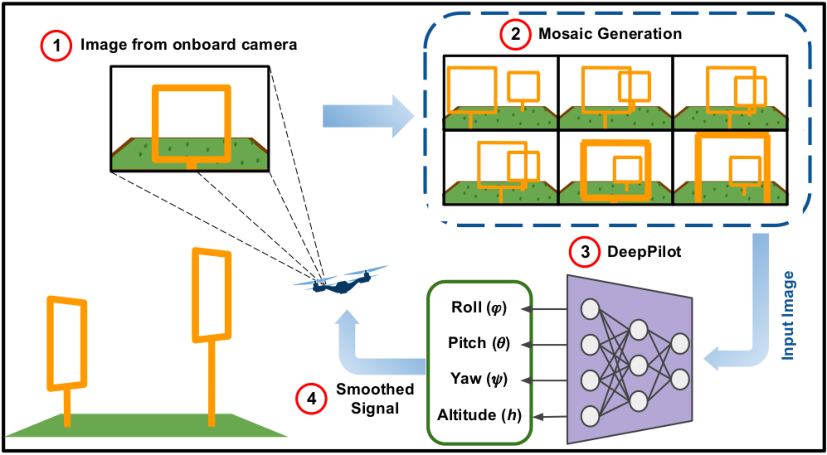
\includegraphics[width=0.7\textwidth]{Rojas_Perez.pdf}
    \caption{Funcionamiento de la red DeepPilot \citet{rojas2020deeppilot}}
    \label{fig:Rojas_Perez}
\end{figure}

En cuanto a soluciones particulares para algoritmos de seguimiento de trayectoria, \citet{foehn2021time} propone una metodología para el cálculo de trayectoria de vuelo en un tiempo óptimo durante el vuelo de un cuadricóptero autónomo, que permite explotar completamente la potencia ofrecida por los actuadores. Además, se plantea una formulación que optimiza la trayectoria de vuelo a lo largo del seguimiento de la trayectoria, se compara la propuesta con otras propuestas y sé válida el algoritmo implementado en un prototipo físico. Por último, se pone a prueba la implementación desarrollada enfrentándola a un piloto de drones experimentado, y los resultados argumentan que la solución implementada logra obtener un desempeño superior al del piloto humano.

\begin{figure}[ht]
    \centering
    \includegraphics[width=0.8\textwidth]{ScienceRobotics21_Foehn.pdf}
    \caption{Funcionamiento de DeepPilot\citet{foehn2021time}}
    \label{fig:Foehn}
\end{figure}

Finalmente, mencionando un ejemplo que va más allá de las competencias de drones autónomos, \citet{stevens2021autonomous} propone el diseño de un quadrotor ligero y dimensiones reducidas, equipado con una serie de sensores y subsistemas que hacen posible su vuelo autónomo en ambientes con alta densidad de vegetación y obstáculos.  La contribución del trabajo se enfoca en el desarrollo del proyecto a partir de requerimientos de efectividad y seguridad, definiendo un diseño de dron que utiliza componentes comerciales de bajo costo. La estimación de estados y la guía de vuelo, generada a través de un sistema de visión artificial, se obtienen a partir de la computadora de vuelo a bordo del vehículo, sin ningún tipo de cálculo previo al vuelo. Además, un sistema de flujo óptico permite sensar la velocidad para la estimación de posición, y los efectos derivados por el derrape se compensan utilizando un GPS.
Los resultados de la implementación demuestran que el sistema propuesto y los algoritmos desarrollados, son capaces de llevar a cabo una evasión dinámica de obstáculos durante el vuelo. La implementación de esta propuesta se realizó tanto en simulación como en físico. La figura \ref{fig:Stevens} muestra el desempeño en simulación del algoritmo de generación de trayectoria propuesto en este trabajo, se realizaron varias pruebas con las trayectorias de vuelo generadas, las trayectorias exitosas son las curvas de color rojo y verde obscuro, mientras que el resto de trayectorias provocaron que el dron chocara con un obstáculo, y se encuentran tachadas en uno de sus extremos.


\begin{figure}[ht]
    \centering
    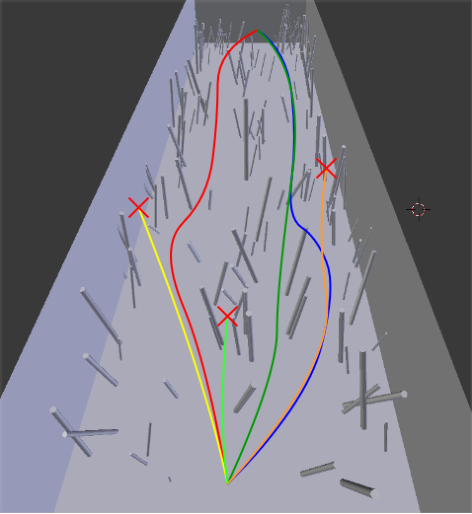
\includegraphics[width=0.5\textwidth]{Stevens_MPhil.pdf}
    \caption{Funcionamiento del algoritmo de gestión de trayectoria desarrollado por \citet{stevens2021autonomous}}
    \label{fig:Stevens}
\end{figure}


A manera de resumen, se analizaron algunos de los algoritmos e implementaciones más sofisticadas hechas en el campo de estudio, al momento de la elaboración de este trabajo. Algunos de los trabajos se enfocaban únicamente en el problema de la detección de compuertas mientras que otros implementaban soluciones específicas para la generación de trayectorias de vuelo, y en otros casos, como los algoritmos desarrollados para las competencias, las implementaciones buscaban superar ambas problemáticas. Por otro lado, en la descripcción de algunos de los trabajos, no se mencionó de forma explícita; sin embargo, la gran mayoría de las propuestas mencionadas pasaron por una etapa de validación llevada a cabo en algún ambiente de simulación, de hecho, algunas de las competencias enfocadas a esta área, evalúan el desempeño de los sistemas propuestos dentro de la simulación como primera etapa para seleccionar a los equipos que participantes, esto se menciona con mayor detalle dentro del marco teórico del presente documento.

Por último, dentro de los ambientes de simulación utilizados por los equipos participantes para entrenar y validar sus algoritmos, existen algunas soluciones bastante especificas enfocadas exclusivamente al vuelo de drones autónomos, tales como FlightGoggle desarrollado por \citet{guerra2019flightgoggles}, Flightmare creado por \citet{song2020flightmare} o AirSim \cite{airsim2017fsr}. Sin embargo, los ambientes anteriores requieren un hardware con poder computacional bastante alto, en especial exigen una tarjeta gráfica dedicada; además, pese a que FlightGoggle y Flightmare ofrecen compatibilidad con ROS, solo lo hacen con ROS 1. En este trabajo se utiliza Gazebo en conjunto con ROS 2 para la implementación de los algoritmos de desarrollados, por lo que se propone un ambiente de simulación abierto que utiliza tecnologías de última generación con requerimientos de hardware básicos.
